\documentclass[10pt,letterpaper]{article}
\usepackage[spanish]{babel}
\usepackage{csquotes}
\usepackage{amsmath,amsfonts,amssymb,mathtools,bm}

% Paquetes de formato e imágenes
\usepackage{graphicx,subfigure}
\usepackage{siunitx} 	% Unidades de medida según SI
\usepackage{booktabs}	% Para el toprule, midrule y bottomrule de las tablas
\usepackage{verbatim}
\usepackage{natbib}     % Requerido para el estilo de bibliografía apalike

% Formato
\usepackage[font=small,labelfont=bf]{caption}
\usepackage[right=2cm,left=2.5cm,top=2.5cm,bottom=2.0cm,headsep=1cm,footskip=1.5cm]{geometry}

% Configuración de la ruta de imágenes
\graphicspath{{figures/}}

% Encabezados e Información del Documento
\title{\textbf{Nota Técnica: Análisis de Deflexión Elástica en una Viga Simplemente Apoyada bajo Carga Centrada}}
\author{David Creutez\\
	{\footnotesize Departamento de Ingeniería en Obras Civiles, Universidad de Santiago de Chile}
}
\date{\today}

% Hipervínculos
\usepackage{hyperref}
\hypersetup{
    colorlinks=true,
    linkcolor=blue,
    citecolor=blue,
    urlcolor=blue,
    pdfauthor = {David Creutez},
    pdftitle = {Nota Técnica: Deflexión de Viga},
    pdfsubject = {Análisis Estructural y Flujo Reproducible}
}

\begin{document}

\maketitle

\section{Introducción, Problema y Objetivos}

Las vigas sometidas a cargas constituyen un caso muy frecuente en la construcción de obras civiles, por lo cual el análisis de cómo se deforman estas estructuras se fundamenta en la teoría de resistencia de materiales y comportamiento elástico de vigas \cite{hibbeler2017mecanica}.

El problema técnico abordado consiste en caracterizar la curva carga-deformación de una viga simplemente apoyada de sección transversal rectangular, sometida a una carga puntual $P$ aplicada en el centro de la luz. El objetivo general es desarrollar un análisis técnico reproducible que permita:
\begin{enumerate}
    \item Realizar un trabajo con las unidades de medida correspondientes en el Sistema Internacional (SI) para llegar a resultados confiables.
    \item Ordenar y estructurar los datos recopilados experimentalmente en una planilla de cálculo Excel (\texttt{Cálculos.xlsx}) junto con las transformaciones de unidades y modelos de cálculo.
    \item Calcular la deflexión teórica según el modelo de Euler-Bernoulli ($\delta_{\text{teo}}$) para cada nivel de carga aplicado.
    \item Comparar los resultados teóricos con los datos experimentales medidos ($\delta_{\text{med}}$).
    \item Mantener la trazabilidad del proceso mediante un flujo de trabajo estructurado en control de versiones utilizando un repositorio sincronizado en GitHub.
\end{enumerate}

\section{Datos y Flujo de Trabajo}

Los datos recibidos en primera instancia fueron ordenados y procesados en un archivo de Excel (\texttt{Cálculos.xlsx}), donde se incluyeron los parámetros geométricos, las conversiones de unidades al Sistema Internacional y la automatización de las fórmulas teóricas. Para garantizar la reproducibilidad y el control de versiones, todo el material del proyecto se integró en un repositorio alojado en GitHub.

\subsection{Transformación de Unidades (SI)}

Para evitar errores dimensionales en la aplicación de las ecuaciones analíticas, se decidió trabajar utilizando las unidades correspondientes al Sistema Internacional. De esta manera, antes de realizar los cálculos, todas las unidades fueron transformadas a sus unidades básicas, evitando el uso de prefijos, abreviaciones o unidades diferentes que pudieran afectar la correcta aplicación de las ecuaciones:

\begin{itemize}
    \item \textbf{Carga puntual ($P$):} Expresada en kilonewtons (\si{\kilo\newton}), convertida a newtons (\si{\newton}):
    \begin{equation}
    P\,[\text{N}] = P\,[\text{kN}] \times 10^3
    \end{equation}
    \item \textbf{Deflexiones ($\delta$):} Medidas en milímetros (\si{\milli\meter}), convertidas a metros (\si{\meter}):
    \begin{equation}
    \delta\,[\text{m}] = \delta\,[\text{mm}] \times 10^{-3}
    \end{equation}
    \item \textbf{Módulo de Elasticidad ($E$):} Expresado en gigapascales (\si{\giga\pascal}), convertido a pascales (\si{\pascal} = \si{\newton\per\meter\squared}):
    \begin{equation}
    E\,[\text{Pa}] = E\,[\text{GPa}] \times 10^9 = 25 \times 10^9 \text{ Pa} = 2.5 \times 10^{10} \text{ Pa}
    \end{equation}
    \item \textbf{Dimensiones geométricas ($b, h, L$):} Homogeneizadas directamente a metros (\si{\meter}).
\end{itemize}

La Tabla~\ref{tab:unidades} resume la correspondencia de factores de conversión empleados en el procesamiento de datos.

\begin{table}[h!]
\centering
\caption{Resumen de conversión de unidades de ingeniería a unidades del Sistema Internacional (SI).}
\label{tab:unidades}
\setlength{\tabcolsep}{4pt}
\resizebox{\textwidth}{!}{%
\begin{tabular}{lcccc}
\toprule
\textbf{Variable} & \textbf{Unidad Origen} & \textbf{Unidad SI} & \textbf{Factor de Conversión} & \textbf{Ejemplo de Entrada} \\
\midrule
Carga ($P$) & \si{\kilo\newton} & \si{\newton} & $\times 10^3$ & $5.0\text{ kN} = 5\,000\text{ N}$ \\
Deflexión ($\delta$) & \si{\milli\meter} & \si{\meter} & $\times 10^{-3}$ & $1.00\text{ mm} = 0.001\text{ m}$ \\
Módulo de Elasticidad ($E$) & \si{\giga\pascal} & \si{\pascal} & $\times 10^9$ & $25.0\text{ GPa} = 2.5 \times 10^{10}\text{ Pa}$ \\
Dimensiones ($b, h, L$) & \si{\meter} & \si{\meter} & $1.0$ & $L = 4.0\text{ m},\, b = 0.2\text{ m},\, h = 0.4\text{ m}$ \\
Inercia ($I$) & \si{\meter^4} & \si{\meter^4} & $1.0$ & $I = 0.001067\text{ m}^4$ \\
\bottomrule
\end{tabular}%
}
\end{table}

Los parámetros geométricos y mecánicos del sistema homogeneizados en unidades SI se recopilan en la Tabla~\ref{tab:parametros}.

\begin{table}[h!]
\centering
\caption{Parámetros geométricos y mecánicos del sistema en unidades SI.}
\label{tab:parametros}
\begin{tabular}{lccc}
\toprule
\textbf{Parámetro} & \textbf{Símbolo} & \textbf{Valor (SI)} & \textbf{Unidades} \\
\midrule
Luz libre & $L$ & \num{4.0} & \si{\meter} \\
Ancho de la sección transversal & $b$ & \num{0.2} & \si{\meter} \\
Altura de la sección transversal & $h$ & \num{0.4} & \si{\meter} \\
Módulo de Elasticidad & $E$ & \num{2.5e10} & \si{\pascal} \\
Segundo momento de área & $I$ & \num{0.001067} & \si{\meter^4} \\
\bottomrule
\end{tabular}
\end{table}

\section{Metodología de Cálculo}

El segundo momento de área (inercia) respecto al eje neutro para la sección rectangular se determina como:
\begin{equation}
I = \frac{b \cdot h^3}{12} = \frac{0.2 \cdot 0.4^3}{12} \approx 0.001067 \text{ m}^4
\end{equation}

La deflexión teórica máxima ($\delta_{\text{teo}}$) en el centro de la luz ($x = L/2$) para una viga simplemente apoyada con carga centrada se obtiene mediante la ecuación clásica de Euler-Bernoulli:
\begin{equation}
\delta_{\text{teo}} = \frac{P \cdot L^3}{48 \cdot E \cdot I}
\end{equation}

Para evaluar la concordancia entre los valores observados ($\delta_{\text{med}}$) y teóricos ($\delta_{\text{teo}}$), se define la diferencia relativa porcentual para cada nivel de carga $P > 0$:
\begin{equation}
\text{Diferencia Relativa (\%)} = \frac{|\delta_{\text{med}} - \delta_{\text{teo}}|}{\delta_{\text{teo}}} \times 100
\end{equation}

Adicionalmente, se monitorea la constancia de la razón $\delta_{\text{med}}/P$ (\si{\milli\meter\per\kilo\newton}) para verificar la respuesta lineal del material.

\section{Resultados y Verificación}

La Figura \ref{fig:carga_deflexion} muestra el gráfico del comportamiento de la deflexión medida frente a la predicción teórica.

\begin{figure}[h!]
\centering
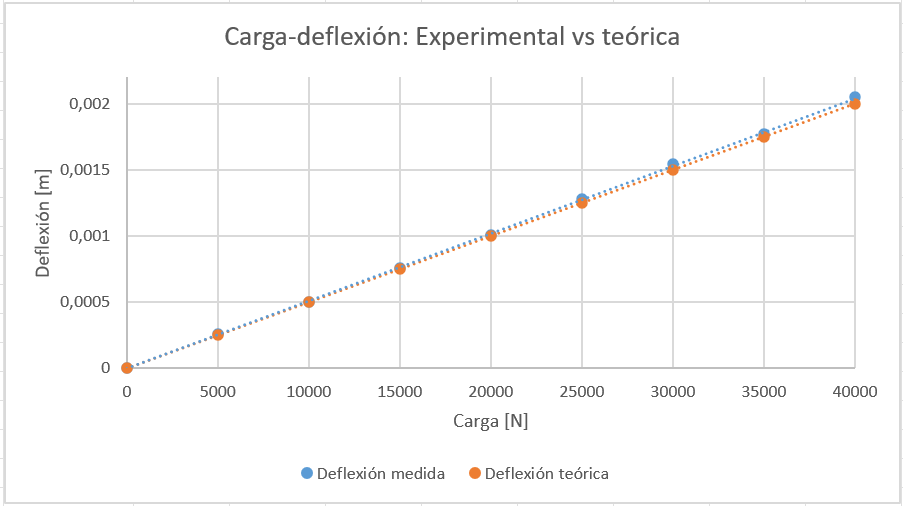
\includegraphics[width=0.75\textwidth]{carga_deflexion.png}
\caption{Comparación entre la deflexión medida y la deflexión teórica en el centro de la luz en función de la carga aplicada.}
\label{fig:carga_deflexion}
\end{figure}

Los resultados numéricos obtenidos a partir de los cálculos fueron extraídos de la planilla de cálculo (\texttt{Cálculos.xlsx}) y expresados en unidades con prefijo por una razón de orden (\si{\kilo\newton} y \si{\milli\meter}) se resumen en la Tabla \ref{tab:resultados}.

\begin{table}[h!]
\centering
\caption{Resumen de resultados de deflexión teórica, medida y verificación de linealidad.}
\label{tab:resultados}
\begin{tabular}{ccccc}
\toprule
\textbf{Carga $P$ [\si{\kilo\newton}]} & \textbf{$\delta_{\text{med}}$ [\si{\milli\meter}]} & \textbf{$\delta_{\text{teo}}$ [\si{\milli\meter}]} & \textbf{Dif. Relativa [\%]} & \textbf{Razón $\delta/P$ [\si{\milli\meter\per\kilo\newton}]} \\
\midrule
0.0  & 0.00 & 0.00 & — & — \\
5.0  & 0.26 & 0.25 & 4.00\% & 0.0520 \\
10.0 & 0.50 & 0.50 & 0.00\% & 0.0500 \\
15.0 & 0.76 & 0.75 & 1.33\% & 0.0507 \\
20.0 & 1.01 & 1.00 & 1.00\% & 0.0505 \\
25.0 & 1.28 & 1.25 & 2.40\% & 0.0512 \\
30.0 & 1.54 & 1.50 & 2.67\% & 0.0513 \\
35.0 & 1.77 & 1.75 & 1.14\% & 0.0506 \\
40.0 & 2.05 & 2.00 & 2.50\% & 0.0513 \\
\bottomrule
\end{tabular}
\end{table}

\section{Interpretación de Resultados}

\begin{enumerate}
    \item \textbf{Ajuste Teórico:} Las diferencias relativas entre los datos medidos y el modelo teórico de Euler-Bernoulli se mantuvieron reducidas en todo el rango ensayado (máximo $4.00\%$ en $P = 5\text{ kN}$), lo que valida la precisión del modelo analítico para esta viga.
    \item \textbf{Respuesta lineal:} La razón $\delta/P$ oscila levemente alrededor de $0.051$~\si{\milli\meter\per\kilo\newton} (entre $0.0500$ y $0.0520$~\si{\milli\meter\per\kilo\newton}), lo que es consistente con un comportamiento lineal de la viga en el intervalo de cargas de $0$ a $40\text{ kN}$.
    \item \textbf{Gestión de Datos y Control de Versiones:} El orden inicial en la planilla Excel (\texttt{Cálculos.xlsx}) facilitó la conversión sistemática a unidades SI. Además, alojar el código y la documentación en un repositorio subido a GitHub asegura la trazabilidad, reproducibilidad y conservación del flujo de trabajo estructural.
\end{enumerate}

\section{Limitación del Flujo de Datos}

A pesar de que el proceso cumple con los estándares de orden y trazabilidad mediante el uso de Excel y GitHub, existen restricciones técnicas ligadas a la automatización del flujo de datos:

\begin{enumerate}
    \item \textbf{Vinculación Manual de Datos:} La transferencia de los resultados numéricos calculados en la planilla \texttt{Cálculos.xlsx} hacia la plantilla de \LaTeX{} se realizó de manera manual sin un script de automatización intermedia, lo que introduce un posible riesgo de descalce ante modificaciones directas en la planilla.
    \item \textbf{Actualización de Archivos Gráficos:} La generación del gráfico explicativo (\texttt{carga\_deflexion.png}) requiere la exportación manual de la imagen previa a la compilación, impidiendo una actualización dinámica en tiempo real del informe técnico frente a cambios en la base de datos.
\end{enumerate}

\section{Conclusiones}

\begin{enumerate}
    \item Se verificó el comportamiento lineal del material dentro del intervalo ensayado ($0\text{ a }40\text{ kN}$), evidenciado por la estabilidad de la razón $\delta/P \approx 0.051\text{ mm/kN}$.
    \item La metodología basada en unidades homogéneas del Sistema Internacional y la estructuración del repositorio en GitHub garantizan la trazabilidad y la reproducibilidad integral del análisis en ingeniería.
\end{enumerate}

\section*{Declaración de Uso de Inteligencia Artificial}

\textbf{Herramientas:} Se utilizaron dos asistentes de IA generativa: Claude (Anthropic) y Gemini (Google).

\textbf{Propósito:} Apoyar el orden y la organización del trabajo, generar la plantilla base en \LaTeX{} y revisar el borrador de la nota técnica, identificando omisiones o inconsistencias respecto al enunciado original.

\textbf{Contenido incorporado:} La estructura de la plantilla en \LaTeX{} (secciones, formato de tablas y figura) junto con sugerencias de organización y redacción que fueron adaptadas tras eliminar inconsistencias. Los datos experimentales, los cálculos de la planilla \texttt{Cálculos.xlsx} y los resultados numéricos fueron elaborados y verificados exclusivamente por el autor.

\textbf{Método de verificación:} Se revisó exhaustivamente cada respuesta emitida por la herramienta de IA, tomando como base los principios teóricos de la mecánica de materiales para aceptar las recomendaciones válidas y descartar cualquier planteamiento erróneo.


% REFERENCIAS BIBLIOGRÁFICAS

\bibliographystyle{apalike}
\bibliography{referencias}

\end{document}

\end{document}


